\documentclass[conference,onecolumn,12pt]{IEEEtran}
\usepackage[english]{babel}
\usepackage{graphicx}
\usepackage{framed}
\usepackage[normalem]{ulem}
\usepackage{amsmath}
\usepackage{listings}
\usepackage{amsthm}
\usepackage{subfigure}
\usepackage{diagbox}
\usepackage{amssymb}
\usepackage{longtable}
\usepackage{palatino}
\usepackage{multirow}
\usepackage{bigstrut}
\usepackage{bbm}
\usepackage{multirow}
\usepackage{algorithm}
\usepackage{booktabs}
\usepackage{algpseudocode} 
\usepackage{amsfonts}
\usepackage[colorlinks,linkcolor=blue,anchorcolor=blue,citecolor=blue]{hyperref}
\usepackage{enumerate}
\usepackage[top=1in,bottom=1in, left=1in, right=1in]{geometry}
\usepackage[utf8]{inputenc}
\usepackage{pgfplots}
\usepgfplotslibrary{groupplots,dateplot}
\usetikzlibrary{patterns,shapes.arrows}
\pgfplotsset{compat=newest}
\newcommand{\R}{\mathbb{R}}
\newcommand{\N}{\mathbb{N}}
\newcommand{\Q}{\mathbb{Q}}
\newcommand{\Z}{\mathbb{Z}}
\numberwithin{equation}{section}
\numberwithin{figure}{section}
\numberwithin{table}{section}

\theoremstyle{definition}
\newtheorem{theorem}{Theorem}
\newtheorem{corollary}{Corollary}
\newtheorem{proposition}{Proposition}
\newtheorem{example}{Example}
\newtheorem{lemma}{Lemma}
\newtheorem*{definition}{Definition}
\newtheorem*{note}{Note}
\newtheorem{exercise}{Exercise}

\newcommand{\Disp}{\displaystyle}
\newcommand{\qe}{\hfill\(\bigtriangledown\)}
\setlength{\columnseprule}{1 pt}
\usepackage{setspace}
\renewcommand{\baselinestretch}{1.5}
\usepackage{fancyhdr}

\begin{document}


\title{{Nonnegative Matrix Factoriaztion}\\
{\footnotesize \textsuperscript{*}Report 3 on the course ``Numerical Optimization".}
}

\author{\IEEEauthorblockN{1\textsuperscript{st} Chen Yihang}
\textit{Peking University}\\
1700010780}

\maketitle


\begin{abstract}
In this report, I give a brief review and implementation of existing nonnegative matrix factoriaztion method. Numerical experiments are performed on synthetic and real-life datasets.
\end{abstract}

\thispagestyle{fancy} % IEEE模板在\maketitle后会自动声明\thispagestyle{plain},
% 导致第一页什么都没有。所以得把plain更改为fancy
\lhead{} % 页眉左,需要东西的话就在{}内添加
\chead{} % 页眉中
\rhead{} % 页眉右
\lfoot{} % 页眉左
\cfoot{} % 页眉中
\cfoot{\thepage} %页眉右,\thepage 表示当前页码
\renewcommand{\headrulewidth}{0pt} %改为0pt即可去掉页眉下面的横线
\renewcommand{\footrulewidth}{1pt} %改为0pt即可去掉页脚上面的横线
\pagestyle{fancy}
\cfoot{\thepage}
\tableofcontents
\clearpage
\section{Introduction}
Given a non-negative matrix
$V$, find non-negative matrix factors $W$ and $H$ such that:
\begin{equation}
  \label{nmf}
  V\approx WH
\end{equation} 
\par We formulate the problem as the following optimization problem:
\begin{equation}
	\label{nmf_opt}
  \begin{split}
    \min \quad f(V,W,H),\quad 
    \text{s.t.}\quad W,H\geq 0
  \end{split}
\end{equation}
\section{Multiplicative update rules}
We briefly introduce multiplicative update rules \cite{NIPS2000_1861}. This paper consider two alternative formulations of NMF, and utilize a rescaled gradient descent on these formulations. The step size is chosen such that the positiveness can be guaranteed every step, and the convergence can be rigorously proved.
\begin{enumerate}
  \item $f(V,W,H)=\|V-WH\|_F^2$. Then a simple additive update rule via gradient descent can be written as 
  \begin{equation}
    \label{additive_1}
    H_{a\mu}\gets H_{a\mu} +\eta_{a\mu}(W^\top V-W^\top W H)_{a\mu}
  \end{equation}
  If we take $\eta_{a\mu}=\frac{H_{a\mu}}{(W^\top W H)_{a\mu}}$, we can get 
  \begin{equation}
    \label{multi_1}
    H_{a\mu}\gets H_{a\mu}\frac{(W^\top V)_{a\mu}}{(W^\top W H)_{a\mu}},\quad W_{ia}\gets W_{ia}\frac{(VH^\top)_{ia}}{(WHH^\top)_{ia}}
  \end{equation}

  \item $f(V,W,H)=D(V\|WH)$. We take the step size to be $\eta_{a\mu}=\frac{H_{a\mu}}{\sum_i W_{ia}}$, the multiplicative rule is
  \begin{equation}
    \label{multi_2}
    H_{a\mu}\gets H_{a\mu} \frac{\sum_i W_{ia}V_{i\mu}/(WH)_{i\mu}}{\sum_k W_{ka}},\quad
    W_{ia}\gets W_{ia}\frac{\sum_\mu H_{a\mu}V_{i\mu}/(WH)_{i\mu}}{\sum_{\mu}H_{a\mu}}
  \end{equation}
\end{enumerate}

In particular, it is straightforward to see that this
multiplicative factor is unity when $V = W H$, so that perfect reconstruction is necessarily a fixed point of the update rules. 

However, despite its theoretical soundness, its performance is subpar compared to another framework, i.e. formulating NMF as an alternating nonnegative least squares problem. 


\section{Nonnegative Least Sqaure Framework}
For simplicity, we consider the following notations in this section:
\begin{equation}
	\min_{H\geq 0} \|V-HW\|_F^2
\end{equation}

There are two groups of algorithms for the NLS problems. The first group consists of the gradient descent and the Newton-type methods that are modified to satisfy the nonnegativity constraints using a projection operator. The second group consists of the active-set and the active-set-like methods, in which zero and nonzero variables are explicitly kept track of and a system of linear equations is solved at each iteration.

\subsection{Projected Gradient Method}

\subsubsection{Vanilla projected gradient method for NMF}
Two projected gradient methods are proposed in \cite{6795860}. In this paper, $f(V,W,H)=\|V-WH\|_F^2$. The author first propose an improved projected gradient method.
For a constraint optimization problem
\begin{equation}
	\begin{split}
		\min_x&\quad f(x)\\
{\rm }&\quad l_i\leq x_i\leq u_i
	\end{split}
\end{equation}

The projected gradient method can be stated as
\begin{equation}
	\label{eq:update_pgd}
	x^{k+1}=P[x^k-\alpha_k\nabla f(x^k)]
\end{equation}
and the full algorithm is stated in Algorithm \ref{alg:pgd}.
\begin{algorithm}
	\caption{Projected gradient method with a back-tracking line search} 
	\begin{algorithmic}[1]
		\State Given $0 < \beta < 1$, $0 < \sigma < 1$. Initialize any feasible $x^1$. Set $\alpha_0=1$.
		\For {$k=1,2,\ldots$}
		\State Assign $\alpha_k\gets \alpha_{k-1}$.
		\If  {$\alpha_k$ satisfies
		\begin{equation}
			\label{eq:pgd}
			f(x^{k+1})-f(x^k)\leq \sigma \nabla f(x^k)^\top (x^{k+1}-x^k)
		\end{equation}}
		repeatedly increase it by $\alpha^k\gets \alpha^k/\beta$ until either the equation is not satisfied or $x(\alpha_k/\beta)=x(\alpha_k)$.
		\Else repeatedly decrease $\alpha_k$ by $\alpha_k\gets \alpha_k \beta$ until $\alpha_k$ satisfies \ref{eq:pgd}.
		\EndIf
		\State Update $x^k$ according to \ref{eq:update_pgd}.
		\EndFor
	\end{algorithmic} 
	\label{alg:pgd}
\end{algorithm}

\paragraph{Alternating Non-negative Least Squares Using Projected Gradient Methods}
We focus on solving
\begin{equation}
	\begin{split}
		\min_H &\quad \tilde{f}(H):=\frac{1}{2}\|V-WH\|_F^2\\
		\text{s.t.}&\quad H\geq 0
	\end{split}
\end{equation}

Since $\tilde{f}$ is quadratic, the equation \ref{eq:pgd} becomes
\begin{equation}
	\label{eq:pgd_trick}
	(1-\sigma)\left<\nabla \tilde{f}(H^k),H^{k+1}-H^k
	\right>+\frac{1}{2}\left<H^{k+1}-H^k, (W^\top W)(H^{k+1}-H^k)
	\right>\leq 0
\end{equation}
which is more computationally efficient. Similarily, we can define $$\bar{f}(W):=\frac{1}{2}\|V^\top - H^\top W^\top \|_F^2$$ and use the identical procedures above.
\paragraph{Directly Applying Projected Gradients to NMF}
We simultaneously update both matrices $(W,H)$ by
\begin{equation}
	(W,H)\gets P[(W,H)-\alpha(\nabla_W f(W,H),\nabla_H f(W,H))]
\end{equation}
and Algorithm \ref{alg:pgd} is applied. Note that since $f$ is not quadratic, we cannot use the trick \ref{eq:pgd_trick} to accelerate the algorithm.

The detailed experiments settings are identical to the paper \cite{6795860}.

\subsubsection{Barzilai-Borwein method for NMF}
A key characteristic of the Barzilai-Borwein method in unconstrained quadratic programming is that the step-length is chosen by a closed-form formula without having to perform a line search:
\begin{equation}
	\begin{split}
		&{x }^{(i+1)}\leftarrow \left[{x }^{(i)}-\alpha ^{(i)}\nabla g({x }^{(i)})\right]_{+}\,\text{ with}\,\,\alpha ^{(i)}=\frac{{s }^{T} s }{{y }^{T} s },\,\text{ where}\\&\quad  s ={x }^{(i)}-{x }^{(i-1)}\,\,\,\text{ and}\,\,\, y =\nabla g({x }^{(i)})-\nabla g({x }^{(i-1)})
	\end{split}
\end{equation}

When the nonnegativity constraints are given, however, back-tracking line search still had to be employed. The nonmonotone line search method proposed in \cite{Raydan} was modified to accommodate the NMF problem. The key difference is that, after an update $\tilde{x}_{k+1}=x_k-\alpha_k g_k$, where $\alpha_k$ is the Barzilai-Borwein step size, we need first project $\tilde{x}_{k+1}$ onto nonnegative vectors, and then perform nonmonotone line search. Several other variants are proposed in \cite{Lixing}, yet the core idea is the same.

\subsubsection{Quasi-Newton method for NMF}
\label{quasi-newton}
Kim et al. \cite{Sra} proposed a quasi-Newton method by utilizing the second order information to improve convergence.

Adopting their notiations, we aim to solve the sub-problem
\begin{equation*}
	\min_{x\geq 0} \frac{1}{2}\|Gx-h\|_F^2
\end{equation*}

They partition
the variables $x$ into two groups, namely the free and fixed variables.
The fixed variables are the components of x with active constraints (equality satisfied) that have a corresponding positive derivative. We index them by the
fixed set, i.e.
\begin{equation}
	I_{+}=\left\{
		i|x_i=0,[\nabla f (x)]_i>0
	\right\}
\end{equation}

Hence, the update can be written as
\begin{equation}
{x }^{i+1}\leftarrow \left(\begin{array}{c} \left[{y }^{i}-\alpha ^{i}{D }^{i}\nabla g({y }^{i})\right]_{+}\\  0 \end{array}\right),
\end{equation}
where $y^{i}$ is a subvector of $x^{i}$ with elements that are not optimal in terms of the Karush–Kuhn–Tucker (KKT) conditions, i.e. not in fixed set $I_{+}$. They efficiently updated $D^{i}$ using the BFGS method and selected $\alpha^{i}$ by a back-tracking line search. Whereas Lin considered a stacked-up problem as in \cite{6795860}, the quasi-Newton method by Kim et al. \cite{Sra} was applied to each column separately. This algorithm is implemented in ``nnls\_pgn.m''. If we apply ``nnls\_pgn.m'' directly, the performace is not satisfactory.

However, their description of exact version of NMF is quite unclear. It is quite confusing how they update the $D$ during Step 3.6 in Algorithm 1. Besides, the stopping condition for the inner loop is also unclear, and I cannot find the authors' implementation to elucidate these points. Hence, I choose to implement the inexact version of quasi-Newton method, i.e. Algorithm 2, FNMA$^{\rm I}$. 
\begin{figure}
	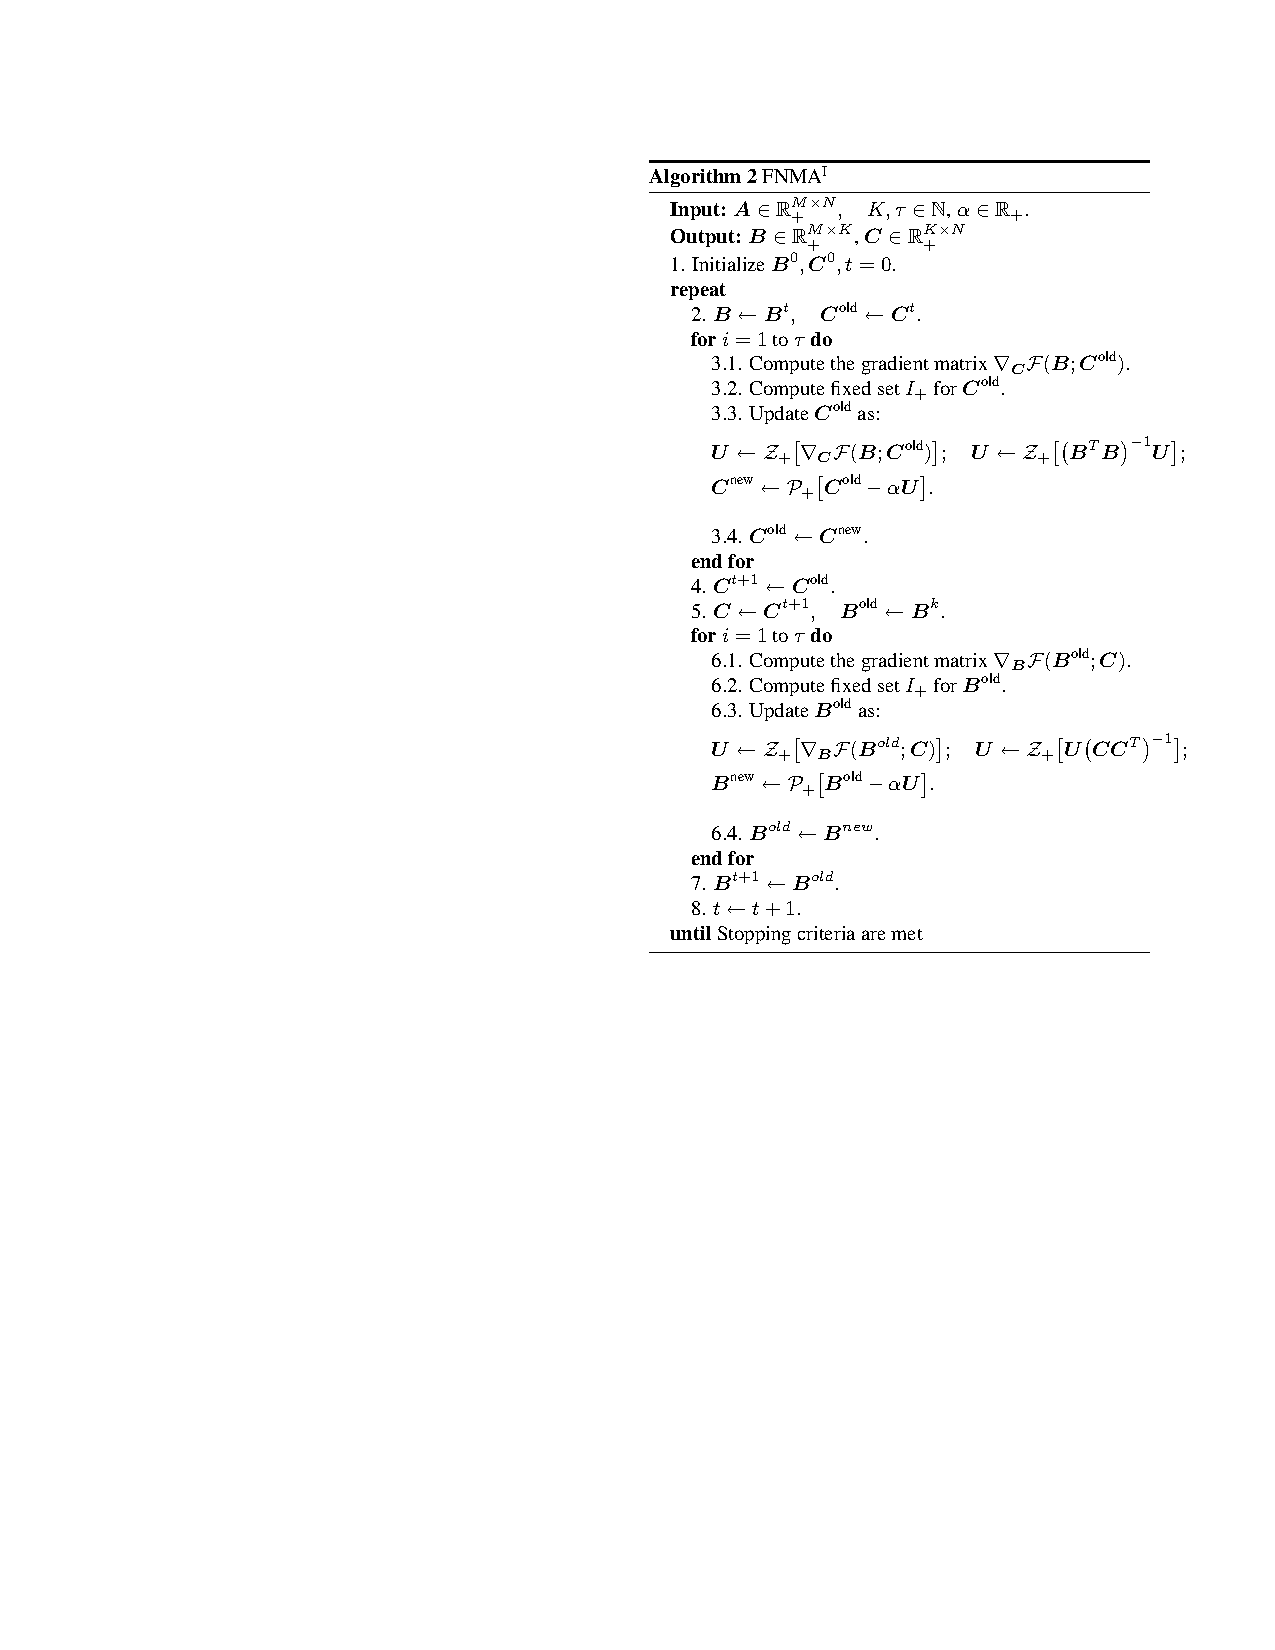
\includegraphics[width=0.6\textwidth]{fi.pdf}
\end{figure}


Details of the algorithm will be presented in the codes but will not be repeatedly stated here. But there are one main difference, I do not adopt its heuristics to choose $\alpha$. Instead, I tune this parameter by hand.

\subsection{Conjugate Gradient method - Proposed method}

I tried to use the conjugate gradient method to solve the subproblem, since it has been proven effective in solving the unconstrained version. I apply the generalized conjugate gradient method \cite{liu1991efficient} on this problem, and test it on various datasets. We find that this idea is not effective, since it is consuming in each iteration. Anyway, I write it in ``nmf\_cg.m''. 

\subsection{Active Set method}
The active-set method for the NLS problems is due to Lawson and Hanson [64]. A key observation is that, if the zero and nonzero elements of the final solution are known in advance, the solution can be easily computed by solving an unconstrained least squares problem for the nonzero variables and setting the rest to zeros. The sets of zero and nonzero variables are referred to as active and passive sets, respectively. In the active-set method, so-called workings sets are kept track of until the optimal active and passive sets are found. A rough pseudo-code for the active-set method is shown in Algorithm 1.

\begin{algorithm}
	\caption{Outline for Active-set method for $\min_{x\geq 0}f(x)=\|Ax-b\|_2^2$} 
	\begin{algorithmic}[1]
		\State Initialize $x$.
		\State Set $\mathcal{I},\mathcal{E}$ to be indices representing zero and nonzero variables. Let $x_{\mathcal{I}}$ and $x_{\mathcal{E}}$ denote the subvectors of $x$ with corresponding indices, and $A_{\mathcal{I}}$ and $A_{\mathcal{E}}$ denote the submatrices of $B$ with corresponding indices.
		\For{$i=1,2,\cdots$}
		\State Solve the unconstrained least squares problem
		\begin{equation}
			\min_{x\geq 0} \|A_{\mathcal{E}}z-b\|_2^2.
		\end{equation}
		\State Check if the solution is nonn and satisfies KKT condition. If so, set $x_{\mathcal{E}}\gets z$, set $x_{\mathcal{I}}$ with zeros, and return $x$. Otherwise, update $x, \mathcal{I},\mathcal{E}$.
		\EndFor
	\end{algorithmic} 
	\label{alg:pgd}
\end{algorithm}

The active-set methods possess a property that the objective function decreases after each iteration; however, maintaining this property often limits its scalability. A main computational burden of the active-set methods is in solving the unconstrained least squares problem; hence, the number of iterations required until termination considerably affects the computation cost. In order to achieve the monotonic decreasing property, typically only one variable is exchanged between working sets per iteration. As a result, when the number of unknowns is large, the number of iterations required for termination grows, slowing down the method. The block principal pivoting method developed by Kim and Park \cite{10.1137/110821172} allows the exchanges of multiple variables between working sets. This method does not maintain the nonnegativity of intermediate vectors nor the monotonic decrease of the objective function, but it requires a smaller number of iterations until termination than the active set methods. It is worth emphasizing that the grouping-based speed-up technique, which was earlier devised for the active-set method, is also effective with the block principal pivoting method for the NMF computation.

\paragraph{NNLS with a single right-hand side vector}
For $\min_{x\geq 0}f(x)=\|Ax-b\|_2^2$, the KKT condition can be written as 
\begin{equation}
	\label{kkt-single}
	y=A^\top Ax-A^\top b,\quad y\geq 0, x\geq 0,\quad x_iy_i=0
\end{equation}

For subset $F$, $G$ of $[n]$, initially, we assign $x_G=0,y_F=0$. The complementary slackness is always satisfied, we can update $x_F,y_G$ via
\begin{subequations}
	\begin{align}
		x_F=\arg\min_{x_F}\|A_Fx_F-b\|_2^2\\
		y_G=A_G^\top (A_Fx_F-b)
	\end{align}
\end{subequations}

If $x,y$ is infeasible, i.e., $x_F\geq 0$ and $y_G\geq 0$ does not hold. Then, we can define $V$ as all the infeasible indices
\begin{equation}
	V=\{i\in F:x_i<0\}\cup\{i\in G:y_i<0\} 
\end{equation}
and choose a subset of $\tilde{V}\subset V$ and the $F,G$ is updated by
\begin{equation}
	F=(F-\tilde{V})\cup (\tilde{V}\cap G),\quad G=(G-\tilde{V})\cup (\tilde{V}\cap F)
\end{equation}
\begin{algorithm}
	\caption{Block principal pivoting method for the NNLS problem with a single right-hand side vector.} 
	\begin{algorithmic}[1]
		\State Initialize $F=\emptyset,G=[n],x=0,y=-A^\top b.\alpha=3,\beta=n+1$.
		\State Update $x_F$ and $y_G$
		\While{$x_F$ and $y_G$ is infeasible}
		\State Compute the infeasible indices set $V$.
		\If {$|V|<\beta$}
		\State Set $\beta=|V|,\alpha=3,\tilde{V}=V$.
		\ElsIf {$|V|\geq \beta$ and $\alpha\geq 1$}
		\State Set $\alpha=\alpha-1,\tilde{V}=V$.
		\ElsIf {$|V|\geq \beta$ and $\alpha=0$}
		\State Set $\tilde{V}$ by $\tilde{V}=\{i:i=\max{i \in V}\}$.
		\EndIf
		\State Update $F,G$. Update $x_F,y_G$.
		\EndWhile
	\end{algorithmic} 
	\label{alg:pgd}
\end{algorithm}

In order to speed up the search procedure, one usually uses $\tilde{V} = V$ , which we call
the full exchange rule. The full exchange rule means that we exchange all variables of
$F$ and $G$ that do not satisfy the KKT condition, and the rule accelerates computation by reducing the
number of iterations required until termination. However, contrary to the active set method in which the variable to exchange is carefully selected to reduce the objective function, the full exchange rule may lead to a cycle and fail to find an optimal solution, though rarely occurs. To ensure finite termination, where only the infeasible variable with the largest index is exchanged,
is a single principal pivoting rule.

\paragraph{NNLS with multiple right-hand side vectors} Now suppose we need to solve the following NNLS problem:
\begin{equation}
	\min_{X\geq 0}\|AX-B\|_F^2
\end{equation}

The process of the single right-hand side vectors are required to perform individually on every column of $B$. 
\subsection{Comparison}
A main difference between the projected iterative methods and the active-set-like methods for the NLS problems lies in their convergence or termination. In projected iterative methods, a sequence of tentative solutions is generated so that an optimal solution is approached in the limit. In practice, one has to somehow stop iterations and return the current estimate, which might be only an approximation of the solution. In the active-set and active-set-like methods, in contrast, there is no concept of a limit point. Tentative solutions are generated with a goal of finding the optimal active and passive set partitioning, which is guaranteed to be found in a finite number of iterations since there are only a finite number of possible active and passive set partitionings. Once the optimal active and passive sets are found, the methods terminate. There are trade-offs of these behavior. While the projected iterative methods may return an approximate solution after a few number of iterations, the active-set and active-set-like methods only return a solution after they terminate. After the termination, however, the solution from the active-set-like methods is an exact solution only subject to numerical rounding errors while the solution from the projected iterative methods might be an approximate one.



\section{Numerical Results}
% Table generated by Excel2LaTeX from sheet 'Sheet1'

\subsection{Stopping codition}
If we take the stopping condition as 
\begin{equation}
	f(W_{k-1},H_{k-1})-f(W_k-H_k)\leq \varepsilon
\end{equation}
the algorithm might be terminated in advance. Hence, we should use the first order optimality condition to formulate a more reasonable stopping condition.

The KKT condition of 
\begin{equation}
	\begin{split}
		\min_{W,H\geq 0} f(W,H) = \frac{1}{2}\|V-WH\|^2_F
	\end{split}
\end{equation}
can be written as
\begin{subequations}
\label{kkt}
	\begin{align}
		& W\geq 0, H\geq 0\\
		& \nabla f_W \geq 0, \nabla f_H\geq 0\\
		& W\odot \nabla f_W = 0, H\odot \nabla f_H  =0
	\end{align}
\end{subequations}

If we define
\begin{equation}
	(\nabla^p f_W)_{mk}:=\begin{cases}
		(\nabla^p f_W)_{mk}\quad & \text{if } (\nabla^p f_W)_{mk}<0 \text{ or } W_{mk}>0\\
	0\quad &\text{otherwise}
	\end{cases}
\end{equation}

$\nabla^p f_H$ is similarly defined. Then the condition \ref{kkt} can be restated as
\begin{equation}
	\nabla^p f_W =0,\text{ and }\nabla^p f_H = 0.
\end{equation}


Hence, we take the stopping condition as
\begin{equation}
	\|\left[\nabla_{W_k} f, (\nabla_{H_k} f)^\top\right]\|_F\leq \varepsilon \|\left[\nabla_{W_0} f, (\nabla_{H_0} f)^\top\right]\|_F
\end{equation}

In the following, we takt $\varepsilon=10^{-4}$.
\subsection{Code description}
\begin{itemize}
	\item nmf\_mu.m: multiplicative weights method.
	\item nmf\_pgd.m: projected gradient method with two variants. The sub-function ``nmf\_subpgd.m'' are excerpted from \cite{6795860}.
	\item nmf\_BB.m: Borwein-Borwein method.
	\item nmf\_newton\_inexact.m: FNMA$^{\rm I}$ in \cite{Sra}.
	\item nmf\_anls.m: active set method with three variants. The sub-function ``anls\_bpp.m'', 'anls\_asgivens.m', 'anls\_asgroup.m', are excerpted from the author's homepage \footnote{https://sites.google.com/site/jingukim/home\#nmfcode}.
	\item png.m: solves the nonnegative least squares problems via quasi-Newton method.
	\item mm\_to\_msm.m: data prepocessing for the ``BBC Sports Datasets''.
	\item display\_image.m: display the face figures.
	\item test.m: performs numerical tests of all the algorithms.
\end{itemize}
\subsection{Test}


In the table, ``rel\_cost'' means $\frac{\|V-WH\|_F}{\|V\|_F}$, and ``rel\_pgn'' means 
$$
\|\left[\nabla_{W_k} f, (\nabla_{H_k} f)^\top\right]\|_F/ \|\left[\nabla_{W_0} f, (\nabla_{H_0} f)^\top\right]\|_F
$$

For the OCR, we take $r=25$, and for the Yale, we take $r=15$, otherwise, we take $r=10$.

There are two main observation:
\begin{enumerate}
	\item If we take all-ones matrices as initial value for PGD type methods. (active set methods cannot take all-ones matrices as initial values).
	\begin{itemize}
		\item PGD-type method and MU is able to terminate after a few steps. However, the solution is not satisfactory in terms of the relative errors, indicating the algorithm falls into a local minima.
		\item On the contrary, the active set method is able to find better solution, despite more iterations are needed.
	\end{itemize}
	\item If we take random matrix as initial vakues, all methods will be able to converge to be close to the global minima. However, the active-set methods still outperforms the PGD-type methods.
\end{enumerate}

In addition, we can discover the following phenonmena:
\begin{itemize}
	\item PGD\_AD outperforms PGD\_Direct. Hence, it favors the alternating scheme.
	\item Geneally, BB is the best project gradient method. While the FNMA-I is very sensitive to the stepsize $\alpha$.
\end{itemize}

{\bf Note}: In this part, proposed method, CG, is not included. While the code is self-contained. I will update the results of CG later.

\paragraph{All-ones init}
The PGD type and MU methods take the initial value of all-one matrices, and the active set methods take the initial value of random matrix.


% Table generated by Excel2LaTeX from sheet 'Sheet1'
\begin{table}[htbp]
	\centering
	\caption{All-ones init, Part 1}
	  \begin{tabular}{clrrrr}
		\toprule
	  \multicolumn{1}{r}{Datasets} & \multicolumn{1}{r}{Method} & iter  & time  & rel\_cost & rel\_pgn \\
	  \midrule
	  \multirow{8}[0]{*}{Rand Mat} & MU    & 2     & 0.0634762 & 0.095014 & 1.25e-07 \\
			& PGD-AD & 3     & 0.1671331 & 0.0950154 & 3.77e-05 \\
			& PGD-Direct & 111   & 5.6326892 & 0.0950165 & 9.58e-05 \\
			& BB    & 1     & 0.0733216 & 0.0950145 & 6.30e-05 \\
			& FNMA-I & 1     & 0.072128 & 0.0950149 & 4.71e-17 \\
			& ANLS-AS-GROUP & 209   & 6.6257293 & 0.0007823 & 9.97e-05 \\
			& ANLS-AS-UPDATE & 180   & 40.1296417 & 0.0010351 & 9.98e-05 \\
			& ANLS-BPP & 334   & 11.5577765 & 0.0006917 & 9.93e-05 \\
			\midrule
	  \multirow{8}[0]{*}{Yale 32 x 32} & MU    & 3     & 0.0244412 & 0.4003346 & 4.51e-06 \\
			& PGD-AD & 6     & 0.0602825 & 0.4003346 & 8.78e-05 \\
			& PGD-Direct & 340   & 2.6615754 & 0.4003347 & 9.95e-05 \\
			& BB    & 5     & 0.045666 & 0.4003346 & 5.31e-05 \\
			& FNMA-I & 1     & 0.0144713 & 0.4004964 & 1.67e-15 \\
			& ANLS-AS-GROUP & 220   & 5.1886074 & 0.2263192 & 9.91e-05 \\
			& ANLS-AS-UPDATE & 234   & 18.1851141 & 0.2263076 & 9.91e-05 \\
			& ANLS-BPP & 129   & 2.3321463 & 0.2262807 & 9.96e-05 \\
			\midrule
	  \multirow{8}[0]{*}{Yale 64 x 64} & MU    & 2     & 0.0448142 & 0.3836777 & 9.39e-05 \\
			& PGD-AD & 5     & 0.1273182 & 0.3836776 & 5.63e-05 \\
			& PGD-Direct & 3730  & 78.0896153 & 0.3836777 & 9.91e-05 \\
			& BB    & 4     & 0.1110037 & 0.3836776 & 1.21e-05 \\
			& FNMA-I & 1     & 0.0517519 & 0.3838597 & 1.73e-15 \\
			& ANLS-AS-GROUP & 82    & 3.2363882 & 0.2025569 & 9.89e-05 \\
			& ANLS-AS-UPDATE & 93    & 21.3143733 & 0.2030481 & 9.98e-05 \\
			& ANLS-BPP & 95    & 3.7758855 & 0.2027377 & 9.99e-05 \\
			\bottomrule
	  \end{tabular}%
	\label{tab:addlabel}%
  \end{table}%

% Table generated by Excel2LaTeX from sheet 'Sheet1'
\begin{table}[htbp]
	\centering
	\caption{All-ones init, Part 2}
	  \begin{tabular}{clrrrr}
		\toprule
	  \multicolumn{1}{r}{Datasets} & \multicolumn{1}{r}{Method} & iter  & time  & rel\_cost & rel\_pgn \\
	  \midrule
	  \multirow{8}[0]{*}{OCR 32 x 32} & MU    & 2     & 0.0179377 & 0.2128464 & 8.61e-06 \\
			& PGD-AD & 6     & 0.1269463 & 0.2128464 & 1.36e-05 \\
			& PGD-Direct & 69    & 1.2389836 & 0.2128465 & 9.49e-05 \\
			& BB    & 2     & 0.0384127 & 0.2128464 & 4.74e-05 \\
			& FNMA-I & 1     & 0.0256251 & 0.2128731 & 2.23e-15 \\
			& ANLS-AS-GROUP & 119   & 4.3202804 & 0.1123091 & 9.94e-05 \\
			& ANLS-AS-UPDATE & 116   & 13.1514948 & 0.1122206 & 9.87e-05 \\
			& ANLS-BPP & 155   & 6.0171304 & 0.1122419 & 9.96e-05 \\
			\midrule
	  \multirow{8}[0]{*}{OCR 32 x 32} & MU    & 2     & 0.0679501 & 0.2138612 & 5.35e-06 \\
			& PGD-AD & 6     & 0.3982755 & 0.2138612 & 7.28e-06 \\
			& PGD-Direct & 743   & 40.701225 & 0.2138612 & 9.83e-05 \\
			& BB    & 4     & 0.6401783 & 0.2138612 & 1.62e-05 \\
			& FNMA-I & 1     & 0.129258 & 0.2138894 & 2.41e-15 \\
			& ANLS-AS-GROUP & 65    & 8.1742325 & 0.1136634 & 9.84e-05 \\
			& ANLS-AS-UPDATE & 89    & 33.4902851 & 0.1139554 & 9.84e-05 \\
			& ANLS-BPP & 72    & 6.84843 & 0.1136423 & 1.00e-04 \\
			\midrule
	  \multirow{8}[0]{*}{BBC sports} & MU    & 3     & 0.1749529 & 0.9377335 & 4.00e-05 \\
			& PGD-AD & 3     & 0.2106645 & 0.9538859 & 9.89e-05 \\
			& PGD-Direct & 0     & 0.0644785 & 0.9897066 & 2.17e-06 \\
			& BB    & 1     & 0.068774 & 0.9537122 & 6.08e-05 \\
			& FNMA-I & 1     & 0.132299 & 0.9408308 & 6.88e-19 \\
			& ANLS-AS-GROUP & 53    & 8.858645 & 0.7764368 & 9.08e-05 \\
			& ANLS-AS-UPDATE & 55    & 35.1259396 & 0.7759689 & 9.70e-05 \\
			& ANLS-BPP & 35    & 4.9804819 & 0.7761014 & 9.21e-05 \\
			\midrule
			\multirow{8}[0]{*}{Text Mining} & MU    & 7     & 0.2343001 & 0.5824757 & 2.80e-05 \\
      & PGD-AD & 8     & 0.3874955 & 0.5826104 & 9.77e-05 \\
      & PGD-Direct & 5000  & 413.1357975 & 0.5121442 & 0.057971158 \\
      & BB    & 5     & 0.4970949 & 0.5826104 & 6.65e-05 \\
      & FNMA-I & 1     & 0.1569973 & 0.7646227 & 3.58e-18 \\
      & ANLS-AS-GROUP & 89    & 7.123137 & 0.1938839 & 9.91e-05 \\
      & ANLS-AS-UPDATE & 122   & 47.2511765 & 0.1943139 & 9.89e-05 \\
      & ANLS-BPP & 106   & 6.7672186 & 0.1943144 & 9.92e-05 \\
			\bottomrule
	  \end{tabular}%
	\label{tab:addlabel}%
  \end{table}%
  
\clearpage
  \paragraph{All-random init}

  All the method take the initial value of random matrix.
  


\begin{table}[htbp]
	\centering
	\caption{All-random init, Part 1}
	  \begin{tabular}{clrrrr}
		\toprule
	  \multicolumn{1}{r}{Datasets} & \multicolumn{1}{r}{Method} & iter  & time  & rel\_cost & rel\_pgn \\
	  \midrule
	  \multirow{8}[0]{*}{Rand Mat} & MU    & 5000  & 1.7994151 & 0.00306886 & 0.001436481 \\
			& PGD-AD & 5000  & 3.3497651 & 0.00310003 & 0.001464601 \\
			& PGD-Direct & 5000  & 2.2137068 & 0.00331001 & 0.001497765 \\
			& BB    & 236   & 0.4001744 & 0.00186104 & 9.92e-05 \\
			& FNMA-I & 2107  & 4.1017117 & 0.00312362 & 1.00e-04 \\
			& ANLS-AS-GROUP & 418   & 0.9321975 & 0.00182876 & 9.95e-05 \\
			& ANLS-AS-UPDATE & 404   & 2.4787843 & 0.00144654 & 9.99e-05 \\
			& ANLS-BPP & 247   & 0.4886891 & 0.00253442 & 9.93e-05 \\
			\midrule
	  \multirow{8}[0]{*}{Yale 32 x 32} & MU    & 5000  & 1.7994151 & 0.00306886 & 0.001436481 \\
			& PGD-AD & 5000  & 3.3497651 & 0.00310003 & 0.001464601 \\
			& PGD-Direct & 5000  & 2.2137068 & 0.00331001 & 0.001497765 \\
			& BB    & 236   & 0.4001744 & 0.00186104 & 9.92e-05 \\
			& FNMA-I & 5000  & 57.0821108 & 0.22646493 & 0.000123439 \\
			& ANLS-AS-GROUP & 173   & 3.195197 & 0.22613218 & 9.95e-05 \\
			& ANLS-AS-UPDATE & 188   & 9.3263954 & 0.22614243 & 9.86e-05 \\
			& ANLS-BPP & 154   & 2.3679411 & 0.2265607 & 9.86e-05 \\
			\midrule
	  \multirow{8}[0]{*}{Yale 64 x 64} & MU    & 5000  & 54.3470377 & 0.20286028 & 0.435776943 \\
			& PGD-AD & 5000  & 111.1331754 & 0.20257292 & 0.085781597 \\
			& PGD-Direct & 5000  & 91.9654021 & 0.26682018 & 0.727151753 \\
			& BB    & 478   & 20.3077045 & 0.20254017 & 9.96e-05 \\
			& FNMA-I & 5000  & 190.5334911 & 0.203118 & 0.001086616 \\
			& ANLS-AS-GROUP & 92    & 3.305792 & 0.20301822 & 9.71e-05 \\
			& ANLS-AS-UPDATE & 97    & 18.6672476 & 0.20293399 & 9.88e-05 \\
			& ANLS-BPP & 112   & 3.9598909 & 0.20239664 & 9.77e-05 \\
			\bottomrule
	  \end{tabular}%
	\label{tab:addlabel}%
  \end{table}%

  % Table generated by Excel2LaTeX from sheet 'Sheet1'
\begin{table}[htbp]
	\centering
	\caption{All-random init, Part 2}
	  \begin{tabular}{clrrrr}
		\toprule
	  \multicolumn{1}{r}{Datasets} & \multicolumn{1}{r}{Method} & iter  & time  & rel\_cost & rel\_pgn \\ \midrule
	  \multirow{8}[0]{*}{OCR 32 x 32} & MU    & 5000  & 42.2873148 & 0.11322416 & 0.068349949 \\
			& PGD-AD & 5000  & 63.4033838 & 0.11196467 & 0.034785003 \\
			& PGD-Direct & 5000  & 75.8243075 & 0.14141454 & 0.123123226 \\
			& BB    & 469   & 17.0553477 & 0.11211716 & 9.95e-05 \\
			& FNMA-I & 5000  & 143.9016236 & 0.1123497 & 0.000223764 \\
			& ANLS-AS-GROUP & 120   & 3.9733914 & 0.11234351 & 9.91e-05 \\
			& ANLS-AS-UPDATE & 110   & 10.9767672 & 0.11227023 & 9.89e-05 \\
			& ANLS-BPP & 141   & 4.4199057 & 0.11245039 & 9.93e-05 \\ \midrule
	  \multirow{8}[0]{*}{OCR 32 x 32} & MU    & 5000  & 143.4988413 & 0.11417625 & 0.078128545 \\
			& PGD-AD & 5000  & 238.2871503 & 0.1132826 & 0.019821524 \\
			& PGD-Direct & 5000  & 279.6411713 & 0.14063169 & 0.131732057 \\
			& BB    & 395   & 39.9729803 & 0.11296143 & 9.93e-05 \\
			& FNMA-I & 5000  & 490.3753745 & 0.1131756 & 0.000137304 \\
			& ANLS-AS-GROUP & 76    & 6.60048 & 0.11398218 & 9.96e-05 \\
			& ANLS-AS-UPDATE & 56    & 18.8935958 & 0.11411991 & 9.93e-05 \\
			& ANLS-BPP & 67    & 5.3393015 & 0.11395586 & 9.95e-05 \\ \midrule
	  \multirow{8}[0]{*}{BBC sports} & MU    & 5000  & 218.01866 & 0.77587115 & 0.005509941 \\
			& PGD-AD & 5000  & 247.5215913 & 0.77666761 & 0.001226171 \\
			& PGD-Direct & 0     & 0.2240347 & 0.98855107 & 4.25e-05 \\
			& BB    & 11    & 0.9722354 & 0.78327213 & 7.56e-05 \\
			& FNMA-I & 68    & 6.9055897 & 0.78639675 & 9.90e-05 \\
			& ANLS-AS-GROUP & 59    & 8.7277818 & 0.77586147 & 9.40e-05 \\
			& ANLS-AS-UPDATE & 48    & 29.0964178 & 0.77610309 & 9.28e-05 \\
			& ANLS-BPP & 53    & 6.5828945 & 0.77610953 & 9.79e-05 \\
			\midrule
			\multirow{8}[0]{*}{Text Mining} & MU    & 5000  & 202.4232239 & 0.1938848 & 0.01067249 \\
			& PGD-AD & 5000  & 263.7314195 & 0.1938804 & 0.065931485 \\
			& PGD-Direct & 5000  & 386.2081692 & 0.1962875 & 0.019447896 \\
			& BB    & 116   & 10.1005863 & 0.1938949 & 1.16e-05 \\
			& FNMA-I & 134   & 9.6698864 & 0.1939238 & 9.94e-05 \\
			& ANLS-AS-GROUP & 152   & 8.8543381 & 0.1943118 & 9.98e-05 \\
			& ANLS-AS-UPDATE & 187   & 70.0897224 & 0.1943113 & 9.24e-05 \\
			& ANLS-BPP & 81    & 4.7091249 & 0.1943113 & 9.96e-05 \\
	  
			\bottomrule

	  \end{tabular}%
	\label{tab:addlabel}%
  \end{table}%
\clearpage

\bibliographystyle{apalike}
\bibliography{bib.bib}




\end{document}
